\newpage
\section{GPU 并行计算}
\subsection{GPU: Graphics Processing Unit}
Originally designed for games.

From simple, fixed, pipline to complex, highly, programmable.

\begin{figure}[!htb]
    \centering
    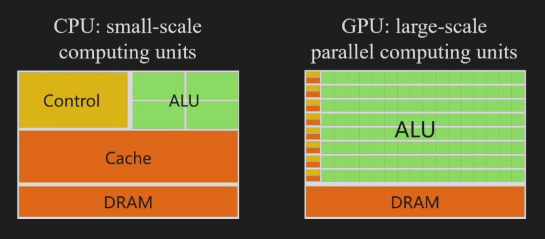
\includegraphics[width=0.42\textwidth]{pic/ACG7/GPU v.s. CPU.png}
    \caption{GPU v.s. CPU}
\end{figure}


\subsection{BSGP: bulk-synchronous GPU programming}
批量同步 GPU 编程语言.

\subsubsection{GPGPU Programming Languages}
Stream processing 流式处理. 
\begin{itemize}
    \item CUDA
    \item OpenCL
    \item DirectX11, Compute Shader
\end{itemize}

\subsubsection{Stream Processing Model}

数据就是流(stream), 流式处理就是以数据为中心.

核函数(kernel), 以流为输入, 核中的指令会并行的作用在流中每一个元素上, 然后形成输出流.

每一个核函数, 会被装载到GPU芯片上.

GPU 本质就是以数据为中心的流式处理器.

\paragraph{Problems}支持高性能, 但是需要好的代码, 让码农头秃. 主要体现在以下方面: 
\begin{itemize}
    \item 影响可读性与可维护性. 
    \subitem 会把语义不相关的代码放在一起, 进行优化, 让代码难以修改. 
    \item 需要手动管理数据流. 
    \subitem 即需要循环利用流, 容易出错.
    \item 代码重用性低
    \subitem 因为核函数是高度特化的, 不能拿过来直接用. 
\end{itemize}

\subsubsection{BSGP}
基于 BSP. 可以以类序列的方式编程.

\paragraph{Example} one-ring neighborhood

计算每个顶点所共享的三角形. 假设有 n 个三角形. 

\begin{enumerate}
    \item 对 3n 个整数排序, 每个三角形会生成三个 32bits 整数, 每个整数对应一个顶点. 整数高16位就是顶点 index, 低 16 位就是三角形 index. 
    \item 排序后, 求出顶点的 index 分隔. 
\end{enumerate}

\begin{code}
    \caption{BSGP}
    \begin{minted}{c++}
        findFaces(int* pf, int* hd, int* ib, int n){
            spawn(n*3){
                rk = thread.rank;   //face id
                f = rk/3;           // vertex id
                v = ib[rk];
                thread.sortby(v);
                // allocate a temp list
                require
                    owner = detmpnew[n]int;
                rk = thread.rank;
                pf[rk] = f;
                owner[rk] = v;
                barrier;
                if(rk == 0 || owner[rk-1] != v)
                    hd[v] = rk;
            }
        }
    \end{minted}
\end{code}

CUDA version 略过.

\subsubsection{BSGP Language Constructs}
\paragraph{结构}\quad
\paragraph{关键字}\quad

会写 complier 会越来越有用, 会写的人也越来越少. 


\subsection{BSGP debuger \& GPU interrupt}
以数据流为中心的调试系统. 

提出 GPU 中断, 让 GPU 可以调用 CPU 函数, 以支持数据流的存储. 


\subsection{Data structures}
\begin{itemize}
    \item Octrees 八叉树, 用以并行的曲面重建, 用点构造 mesh
    \item KD-Trees
    \item 6D Spatial Hierarchies
\end{itemize}
\subsection{Applications}
摸了